\documentclass[12pt]{article}
\usepackage[margin=1in]{geometry} 
\usepackage{amsmath,amsthm,amssymb,amsfonts}
\usepackage{romannum}
\usepackage{dsfont}
\usepackage{graphicx}
 
\newcommand{\N}{\mathbb{N}}
\newcommand{\Z}{\mathbb{Z}}
 
\newenvironment{problem}[2][Problem]{\begin{trivlist}
\item[\hskip \labelsep {\bfseries #1}\hskip \labelsep {\bfseries #2.}]}{\end{trivlist}}
%If you want to title your bold things something different just make another thing exactly like this but replace "problem" with the name of the thing you want, like theorem or lemma or whatever

\renewcommand\thesubsubsection{\arabic{subsubsection}}
 
\begin{document}
 
%\renewcommand{\qedsymbol}{\filledbox}
%Good resources for looking up how to do stuff:
%Binary operators: http://www.access2science.com/latex/Binary.html
%General help: http://en.wikibooks.org/wiki/LaTeX/Mathematics
%Or just google stuff
 
\title{Localization \Romannum{1}}
\date{\vspace{-20mm}}
\maketitle

\section*{Map-based localization} 

\subsection*{Robot localization problem}

This exercise is designed to exercise your understanding of the basics of the SEE-ACT cycle together with the belief update.

\subsubsection{ACT phase}

Imagine that we are dealing with a robot in a 1D environment. The initial position of the robot, $\vec{x}_0$ is known with probability $Pr=1.0$. The following diagram presents the initial robot setup: \\

\begin{figure}[h]
\noindent\makebox[\textwidth]{
	\centering
	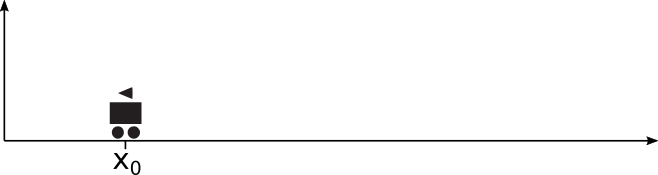
\includegraphics[width=0.8\linewidth]{loc1_robot_x0}
}
\end{figure}

Let's imagine now that our robot has done two consecutive forward movements (up to x1 and x2, respectively). \\

\begin{figure}[h]
\noindent\makebox[\textwidth]{
	\centering
	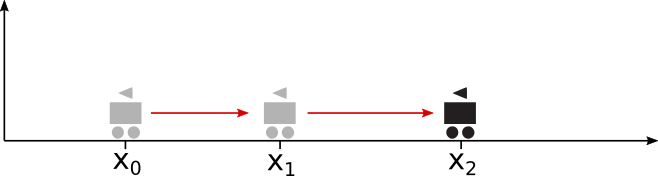
\includegraphics[width=0.8\linewidth]{loc1_robot_move}
}
\end{figure}

Which of the following diagrams represents the robot's belief about its positions based on the wheel odometry measurements (presented as a probability density function)?

\pagebreak

\subsubsection*{Answer}

\begin{figure}[h]
\noindent\makebox[\textwidth]{
	\centering
	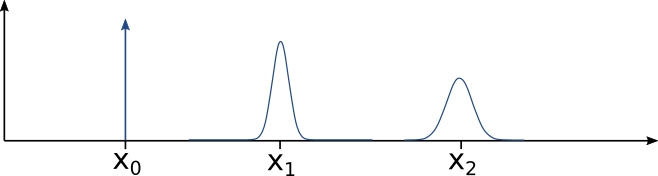
\includegraphics[width=0.8\linewidth]{loc1_odo_belief2}
}
\end{figure}

\noindent As robot acts, it estimates the position by odometry using \textbf{proprioceptive sensors}(e.g. encoders) and uncertainty of the position increases. Note that we know the exact initial position of robot thus $\vec{x}_0$ can be represented as a delta function. 


\subsubsection{SEE phase}

The robot completed the ACT phase with a certain belief that will be now denoted as $\vec{x}_{odo}$. \\

\noindent In the SEE stage the robot is using a built-in laser rangefinder with a non-zero uncertainty. The rangefiner reports that there is a wall at distance $x$ in front of the robot: \\ 

\begin{figure}[h]
\noindent\makebox[\textwidth]{
	\centering
	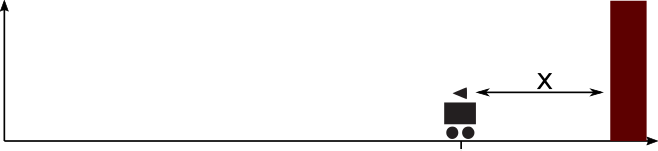
\includegraphics[width=0.8\linewidth]{loc1_robot_see}
}
\end{figure}

\noindent Assuming that a map of the environment is available, what will the belief of the robot be based only on the rangefinder measurement (i.e. before the belief update and fusion with the odometry information)?

\subsubsection*{Answer}

The robot using \textbf{exteroceptive sensors}(e.g. camera, laser rangefinder etc) to estimate the position.

\begin{figure}[h]
\noindent\makebox[\textwidth]{
	\centering
	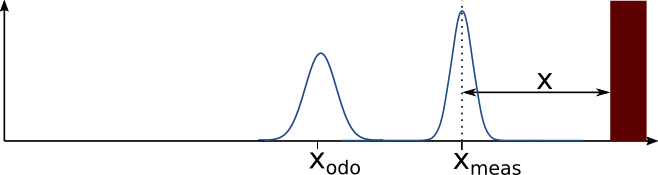
\includegraphics[width=0.8\linewidth]{loc1_meas_belief1}
}
\end{figure}


\pagebreak

\subsubsection{Belief update (information fusion)}

After completing the ACT stage and the SEE stage, it is time to fuse the information the robot gathered. We should perform a perception update on top of the odometry estimate to compute a single, statistically correct belief. \\

\noindent We start the belief update process with with an odometry estimate, $\vec{x}_{odo}$, and a measurement estimate, $\vec{x}_{meas}$: \\

\begin{figure}[h]
\noindent\makebox[\textwidth]{
	\centering
	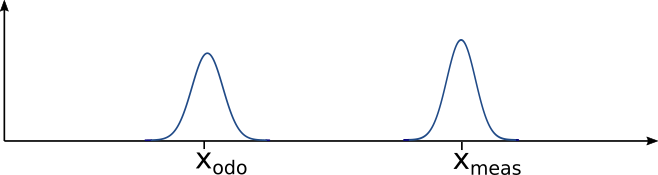
\includegraphics[width=0.8\linewidth]{loc1_fusion_input}
}
\end{figure}

What is the expected probability density function of the resulting belief $\vec{x}_{posterior}$?

\subsubsection*{Answer}

By fusion of two pdf, resulting probability density function has small variance (high peak).

\begin{figure}[h]
\noindent\makebox[\textwidth]{
	\centering
	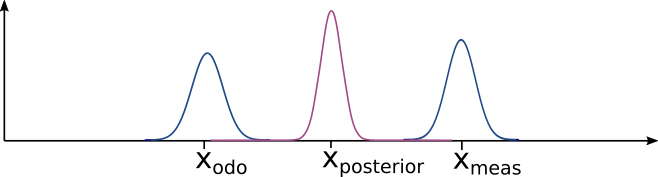
\includegraphics[width=0.8\linewidth]{loc1_fusion_belief1}
}
\end{figure}

\end{document}